\documentclass[a4paper, 12pt]{article} % тип документа

%%%Библиотеки
    %\usepackage[warn]{mathtext}	
    \usepackage[T2A]{fontenc}   %Кодировка
    \usepackage[utf8]{inputenc} %Кодировка исходного текста
    \usepackage[english, russian]{babel} %Локализация и переносы
    \usepackage{caption}
    \usepackage{listings}
    \usepackage{amsmath, amsfonts, amssymb, amsthm, mathtools}
    \usepackage[warn]{mathtext}
    \usepackage[mathscr]{eucal}
    \usepackage{wasysym}
    \usepackage{graphicx} %Вставка картинок правильная
    \usepackage{indentfirst}
    \usepackage{float}    %Плавающие картинки
    \usepackage{wrapfig}  %Обтекание фигур (таблиц, картинок и прочего)
    \usepackage{fancyhdr} %Загрузим пакет
    \usepackage{lscape}
    \usepackage{xcolor}
    \usepackage[normalem]{ulem}
    
    \usepackage{titlesec}
    \titlelabel{\thetitle.\quad}

    \usepackage{hyperref}

%%%Конец библиотек

%%%Настройка ссылок
    \hypersetup
    {
        colorlinks = true,
        linkcolor  = blue,
        filecolor  = magenta,
        urlcolor   = blue
    }
%%%Конец настройки ссылок


%%%Настройка колонтитулы
    \pagestyle{fancy}
    \fancyhead{}
    \fancyhead[L]{2.2.1}
    \fancyhead[R]{Глаз Роман, группа Б01-007}
    \fancyfoot[C]{\thepage}
%%%конец настройки колонтитулы



\begin{document}
                        %%%%Начало документа%%%%


%%%Начало титульника
\begin{titlepage}

    \newpage
    \begin{center}
        \normalsize Московский физико-технический институт \\(госудраственный университет)
    \end{center}

    \vspace{6em}

    \begin{center}
        \Large Лабораторная работа по общему курсу физики\\Термодинамика и молекулярная физика
    \end{center}

    \vspace{1em}

    \begin{center}
        \Large \textbf{2.2.1. Исследование диффузии газов}
    \end{center}

    \vspace{2em}

    \begin{center}
        \large Глаз Роман Сергеевич\\
        Группа Б01-007
    \end{center}

    \vspace{\fill}

    \begin{center}
        Долгопрудный \\2021
    \end{center}
    
\end{titlepage}
%%%Конец Титульника



%%%Настройка оглавления и нумерации страниц
    \thispagestyle{empty}
    \newpage
    \tableofcontents
    \newpage
    \setcounter{page}{1}
%%%Настройка оглавления и нумерации страниц


                    %%%%%%Начало работы с текстом%%%%%%

\textbf{Цель работы:} регистрация зависимости концентрации гелия в воздухе от времени с помощью датчиков теплопроводности при разных начальных давлениях смеси газов. Определение коэффициента диффузии по результатам измерений.\\

\textbf{Используемое оборудование:} измерительная установка, форвакуумный насос, баллон с газом (гелий), манометр, источник питания, магазин сопротивлений, гальваномет.

\section{Теоретическое введение}

Диффузия -- самопроизвольное взаимное проникновение веществ друг в друга, происходящее вследствие хаотичного теплового движения молекул. При перемешивании молекул разного сорта говорят о взаимной (или концентрационной) диффузии.

В системе, состоящей из двух компонентов, плотность потока вещества в результате взаимной диффузии описывается законом Фика:

\begin{equation}
    j_a = -D_{ab} \frac{\partial n_a}{\partial x} \text{, }j_b = -D_{ba} \frac{\partial n_b}{\partial x},
\end{equation}
где $D_{ba} = D_{ab} = D$ -- коэффициент взаимной диффузии компонентов, $j_{a,b}$ = плотности потока частиц соответствующего сорта (количество частиц, пересекающих единичную площадку в единицу времени).


В работе исследуется диффузия примеси лёгкого газа (гелия) на фоне воздуха, поэтому концентрация воздуха в опыте значительно больше концентрации гелия, и её относительное изменение незначительно. В процессе работы будет описываться только диффузия примеси гелия на стационарном фоне воздуха.

Проведём теоретическую оценку величины коэффициента взаимной диффузии. В работа мала концентрация гелия, более того, масса атомов гелия много меньше массы молекул, составляющих воздух. При таких условиях перемешивание газов в эксперимента можно рассматривать как диффузию гелия на стационарном форне воздуха. Тогда коэффициент диффузии приблизительно равен

\begin{equation}
    D = \frac{1}{3}\lambda \bar v,
\end{equation}

где $\lambda$ - длина свободного пробега частиц гелия, $\bar v = \sqrt{\frac{8kT}{\pi m}}$ -- их средняя тепловая скорость. В общем случае необходимо считать $\lambda = \frac{1}{n_\Sigma \sigma}$, где $n_\Sigma = n_{He} + n_B = \frac{P_\Sigma}{kT}$ - полная концентрация частиц, $\sigma$ -  среднее сечение столкновения частиц гелия с воздухом. Также  $\bar v = \sqrt{\frac{8kT}{\pi \mu}}$ - средняя относитель. Таким образом, теоретическая оценка предполагает, что коэффициент диффузии не зависит от пропорция элементов, а обратно пропорционален давлению $D \propto \frac{1}{P_\Sigma}$.

Рассмотрим процесс выравнивания концентрации в установке, она зависит от координат и времени во всей установке. Объём соединительной трубки мал по сравнению с с объёмами сосудов. Поэтому концентрации газов можно считать постоянной по всему объёму сосудов; считаем, что процесс выравнивания происходит только за счёт диффузии в трубке и является стационарным (так как считаем стационарным поток частиц). Величина этого стационарного потока $J = -DS\frac{\partial n}{\partial x}$, и он одинаковый во всём сечении трубки, тогда $n(x)$ - линейная функция координаты и $\frac{dn}{dx} = \frac{\triangle n}{l}$ ($l$ -- длина трубки), получаем 

\begin{equation}
    J = -DS \left( \frac{n_1-n_2}{l} \right)
\end{equation}

Предположим, что установился линейный профиль концентрации и полученное соотношение справедливо в любой момент времени. Получаем квазистационарное приближение зависимости концентраций $n_1$ и $n_2$ от времени.

Через $\triangle n_1$ и $\triangle n_2$ обозначим изменения концентрации в объёмах $V_1$ и $V_1$ за время $\triangle t$. Тогда $V_1 \triangle n_1$ - изменение количества компонента в объёме $V_1$, а $V_2 \triangle n_2$ - изменение количества этого компонента в объёме $V_2$. По закону сохранения вещества следует, что $V_1 \triangle n_1 + V_2 \triangle n_2 = const$, поэтому $V_1 \triangle n_1 = - V_2 \triangle n_2$. Эти изменения происходят вследствие диффузии, поэтому

\begin{equation}
    V_1 \triangle n_1 = - V_2 \triangle n_2 = J \triangle t = -DS   \left( \frac{n_1-n_2}{l} \right) \triangle t
\end{equation}

Делим равенство на $\triangle t$

\begin{equation}
    V_1 \frac{dn_1}{dt} = -DS \left( \frac{n_1-n_2}{l} \right) \text{, } V_2 \frac{dn_2}{dt} = -DS \left( \frac{n_1-n_2}{l}\right)
\end{equation}

Делим первое уравнение на $V_1$, второе на $V_2$, вычтем равенства друг из друга:

\begin{equation}
    \frac{dn_1}{dt}- \frac{dn_2}{dt} = - \frac{n_1-n_2}{l}DS \left( \frac{1}{V_1} +\frac{1}{V_2} \right)
\end{equation}

Введём новую переменную $\triangle n = n_1-n_2$, проинтегрируем уравнение, получим

\begin{equation}
    \triangle n = \triangle n_0 e^{\frac{-t}{\tau}},
\end{equation}
где $\triangle n_0$ - разность концентраций примеси в начльный момент времени, а

\begin{equation}
    \tau = \frac{V_1 V_2}{V_1 + V_2} \frac {l}{SD}
\end{equation}

Видим, что разность концентраций убывает по экспоненциальному закону и тем быстрее, чем меньше $\tau$ - величина, определяющаяся геометрическими параметрами установки и величиной коэффициента диффузии.

Для проверки применимости квазистационарного течения убедимся, что время $\tau$ много больше характерного времени диффузии одной частицы вдоль трубки длиной l: $t_{diff} \sim \frac{l^2}{D} \ll \tau$.

Для измерения концентраций применяются датчики теплопроводности $D_1$ и $D_2$ (см. рис. 1) и используется зависимость теплопроводности газовой смеси от её состава. Тонкая проволока радиуса $r$, протянутая вдоль оси цилиндра радиуса $R$, нагревается током. Тепло от проволоки к стенке цилиндра передаётся главным образом впоследствие теплороводности газа, находящегося внутри цилиндра. Количество тепла переданного стенке цилиндра в единицу времени, определяется по формуле

\begin{equation}
    Q = \kappa \frac{2\pi L}{ln (R/r)}(T_1-T_2),
\end{equation}

где $\kappa$ - теплопроводность, $L$ - длина нити, $T_1, T_2$ - температуры проволочки и стенки. При $Q = const$ температура проволоки и её сопротивление определяются теплопроводностью газа и, следовательно, его составом. Для измерения разности концентраций газов используется  
мостовая схема, представленная на рис. 2 (см. пункт 4).

В процессе диффузии разность концентраций убывает по экспоненциальному закону. По тому же закону изменяются во времени показания гальванометра:

\begin{equation}
    U = U_0 e^{\frac{-t}{\tau}}
\end{equation}

Измеряя экспериментально зависимость $U(t)$, можно получить характерное время процесса $\tau$, откуда определить коэффициент диффузии $D$.

\section{Экспериментальная установка}

Общий вид конструкции установки приведён на рис. 1. Установка состоит из двух сосудов $V_1$ и $V_2$, соединённых краном $K_3$, форвакуумного насоса Ф.Н. с выключателем $Т$, манометра $М$ и системы напуска гелия, состоящей из кранов $K_6, K'_6, K_7$. Кран $K_5$ позволяет соединять форвакуумны насос либо с установкой, либо с атмосферой. Сосуды $V_1$ и $V_2$ соединены трубкой длины $l$ и сечения $S$. Сосуды заполнены смесь двух газов при одинаковом давлении, но с различной концентрацией компонентов. Вследствие взаимной диффузии концентрации каждого из компонентов с течением времени выравниваются Между форвакуумным насосом и краном $K_5$ вставлен предохранительный баллон, защищающий кран и установку при неправильной её эксплуатации от попадания форвакуумного масла из насоса. Сосуды $V_1$ и $V_2$ можно соединять как с системой напуска гелия, так и с форвакуумным насосом. Для этот служат краны $K_1, K_2, K_4, K_5$. Манометр М регистрирует давление газа, до которого заполняют тот или иной сосуды. Кран $K_4$ изолирует форвакуумный насос от установки. Для подачи воздуха в установку служит кран $K_5$. Дополнительный кран $K'_6$ служит для вакуумной изоляции установки от системы подачи гелия. Краны $K_4, K_5, K'_6$ обладают повышенной вакуумплотностью и хорошо изолируют установку от протечек.

\begin{figure}[h]
    \centering
    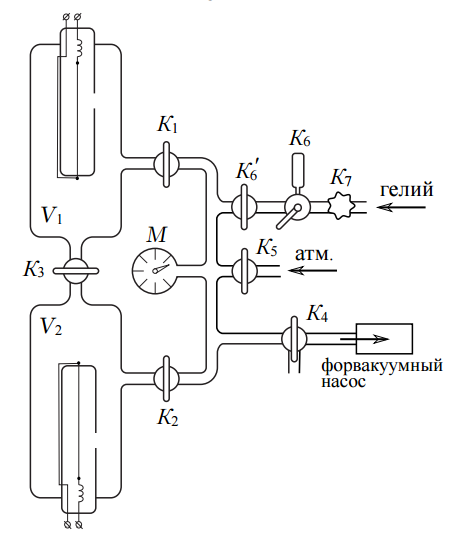
\includegraphics[width = 7.5 cm]{facility.png}
    \caption{Установка для исследования взаимной диффузии газов}
    \label{fig:vac}
\end{figure}

Для измерения разности концентраций газов используется мостовая схема, представленная на рисунке 2.

Здесь $D_1, D_2$ - датчики теплопроводности, расположенные в сосудах $V_1$ и $V_2$. Сопротивления $R_1, R_2, R$ служат для установки прибора на нуль (балансировка моста). В одну из диагоналей моста включен гальванометр, к другой подключается небольшое постоянное напряжение. Сопротивления $R_1$ и $R_2$ спарены (их подвижные контакты находятся на общей оси) и изменяются одновременно при повороте ручки грубой регулировки. Точная балансировка выполняется потенциометром R. Балансировку необходимо проводить перед каждым экспериментом заново: при этом установка заполняется чистым газом (воздухом без гелия) при давлении, близком «рабочему» (при котором затем будут проводится измерения).

Мост балансируется при заполнении сосудов (и датчиков) одной и той же смесью. При заполнении сосудов смесями различного состава возникает «разбаланc» моста. При незначительном различии в составах смесей показания гальванометра, подсоединённого к диагонали моста, будут пропорциональны разности концентраций примеси: $U \propto \triangle \kappa \propto \triangle n$
 
\begin{figure}[h]
    \centering
    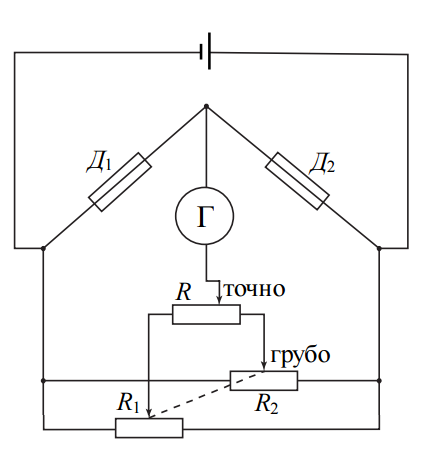
\includegraphics[width = 5.5 cm]{scheme.png}
    \caption{Мостовая схема с датчиками теплопроводности для измерения разности концентраций газов}
    \label{fig:vac}
\end{figure} 

Гелий содержится в баллоне (не изображен на рис. 1) под давлением, превышающим атмосферное. Для предотвращения избыточного расхода гелия и
его неконтролируемого проникания в установку предусмотрен металлический кран ($K_7$), отделяющий её от баллона с гелием. Его открывают только на
время непосредственного заполнения установки гелием, остальное время он должен быть закрыт. Для подачи малых порций гелия предусмотрен двухходовый кран с дозатором (рис. 4). При повороте рычажка $Р$ в положение $I$ гелий в небольшом количестве поступает в дозатор (если открыт $К_7$), а при повороте $Р$ в положение $II$ порция из дозатора поступает в установку.

\begin{figure}[h]
    \centering
    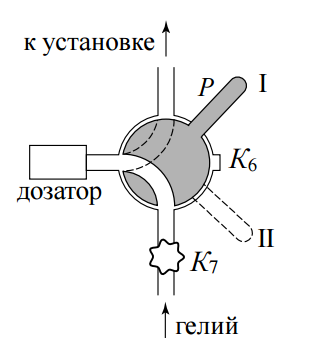
\includegraphics[width = 5.5 cm]{crane.png}
    \caption{Кран $K_6$}
    \label{fig:vac}
\end{figure} 

\section {Ход работы}

Изучим схему установки и инструкции по откачке воздуха, напуске гелия и откачке воздуха для конкретной установки. Ознакомимся с расчётной программой, используемой для считывания данных с датчиков теплопроводности. 

Включим питание датчиков теплопроводности и измерительного моста. Убедимся, что краны подачи гелия $K_7, K'_6$ плотно закрыты. Откачаем установку до давления $\sim 0,1$ Торр. Для этого

\begin{itemize}
\item закроем краны $K_4, K_5, K'_6$;
\item включим насос тумблером (расположен на насосе) и дадим ему откачать собственный объём ($\sim $3–5 с);
\item откроем кран $K_4$, соединив с его помощью насос и установку;
\item спустя 3-5 минут остановим откачку: отделим насос от установки краном $K_4$;
\item выключим насос тумблером (насос снабжен встроенным обратным клапаном, препятствующим выбросу масла после остановки, поэтому соединять насос с атмосферой необходимости нет)
\end{itemize}

Сбалансируем измерительный мост при предполагаемом «рабочем»
давлении (суммарном давлении смеси в эксперименте). В качестве начального рабочего давления возьмём $P_\Sigma \sim$ 40 торр. Для этого

\begin{itemize}
\item подадим воздух краном $K_5$ непосредственно из атмосферы
\item изолируем рабочие объёмы кранами $K_1, K_2$ ($K_3$ открыт)
\item сбалансируем измерительный мост так, чтобы показания вольтметра флуктуировали в среднем около нулевого значения. Используем последовательно ручки регулировки «грубо», затем «точно». По достижении баланса переключатели моста установим на максимум. Диапазон измерений гальванометра переведём на 10мкА После балансировки и до окончания измерений при данном $P_\Sigma$ положения ручек регулировки не меняются
\end{itemize}

Заполним установку рабочей смесью: в сосуде $V_1$ находится воздух, а в сосуде $V_2$ - смесь воздуха с гелием. Давление должно быть одинаковым и равным рабочему давлению $P_\Sigma$. Заполнение производится в следующем порядке:

\begin{itemize}
\item откачаем всю установку до $\sim$ 0,1 Торр
\item изолируем объём $V_1$, закрыв краны $K_1$ и $K_3$ (туда не должен попасть гелий!). После этого остановим откачку
\item напустим в установку гелий до давления $P_{He} = 0,1 P_{\Sigma}$. Избыточное количество гелия при необходимости откачаем насосом. После этого изолируйте объём $V_2$ (краном $K_2$).
\item перекроем подачу гелия (кран $K_7$) и откачаем гелий из всех патрубков. После чего остановим откачку.
\item присоединим объём $V_1$ к установке (кран $K_1$) и заполним всю установку, исключая объём $V_2$, воздухом (без гелия) до несколько избыточного по сравнению с рабочим давления ($\sim 1,5 P_{\Sigma} $ в зависимости от соотношения объёмов патрубков и сосудов.
\item уравняем давление в сосудах $V_1$ и $V_2$, направив поток воздуха с избыточным давлением в сосуд с гелием. Для этого откроем кран $K_2$
при уже открытом $K_1$ (кран $K_3$ всё ещё закрыт!) Поскольку газ при адиабатическом расширении остывает, необходимо держать краны $K_1$ и $K_2$ открытыми в течение некоторого времени ($30-60$ с), чтобы дать давлениям выравняться при одинаковых температурах. Это время не должно быть слишком велико, чтобы диффузия гелия по патрубкам не привела к искажению приготовленного состояния.
\item запишем точное значение установившегося рабочего давления $P_\Sigma$. Изолируем объёмы $V_1$ и $V_2$, перекрыв краны $K_1$ и $K_2$. Система должна быть готова к измерениям.
\end{itemize}

Процесс диффузии начнётся после открывания крана $K_3$ . Приготовим компьютерную программу по дополнительному описанию. Откроем $K_3$ и измерим, как меняются показания вольтметра с течением времени $U(t)$. Измерение будем продолжать до тех пор, пока напряжение не упадет хотя бы на 30–50\%.

Повторим измерения предыдщуих пунктов $2 - 6$ при различных значениях рабочего давления в диапазоне $40 - 300$ торр. Результаты измерений, снятые с компьтера, занесём в таблицу (см. приложения).

Построим графики зависимостей непосредственно изменений показания вольметра от времени. Некоторые эксперименты получились неудачными, из-за чего учитывать их не будем. 

Построим графики зависисмотей показаний вольтметра от времени в логарифмическом масштабе. Теория предсказывает, что характер зависимости - обратная пропорциональность, модуль углового коэффициента уменьшается с повышением давления. 

Значения коэффициентов наклона и их погрешности определим по методу наименьших квадратов:

\begin{equation}
    \sigma_k = \frac{1}{\sqrt{n}}\sqrt{\frac{<ln U^2>-<ln U>^2}{<t^2>-<t>^2}-k^2}
\end{equation}

Коэффициент диффузии рассчитывается по формуле $D = -\frac{kVL}{2S}$, его ошибка будет составлять $\sigma_D = D\sqrt{(\frac{\sigma_V}{V})^2+(\frac{\sigma_k}{k})^2+(\frac{\sigma_L/S}{L/S})^2}$

Параметры установки: $V = 360 \pm 0,5 cm^3$, $L/S = (7,0 \pm 0,5) \frac{1}{cm}$.

\begin{center}
    \begin{tabular}{|c|c|c|c|c|c|}
        \hline 
        $P, \text{Торр}$ & $\frac{10^{-4}}{P}, \frac{1}{\text{Торр}}$ & $-k \cdot 10^{-3}, \frac{1}{c}$ & $\varepsilon_{k}$ & $D, \frac{cm^2}{c}$ & $\varepsilon_{D}$ \\ 
        \hline 
        55 & 180 & 8,26 & 0,037 & 10,40 & 0,080 \\ 
        \hline 
        169 & 59 & 2,76 & 0,011 & 3,48 & 0,072 \\ 
        \hline 
        200 & 50 & 2,33 & 0,013 & 1,97 & 0,072 \\ 
        \hline 
        293 & 34 & 1,63 & 0,058 & 1,35 & 0,092 \\ 
        \hline 
        447 & 22 & 1,11 & 0,073 & 0,92 & 0,102 \\ 
        \hline 
    \end{tabular} 
\end{center}

Теперь убедимся в применимости модели квазистационарного приближения. Для этого должно выполняться то, что время процесса $\tau$ много больше характерного времени диффузии отдельной частицы вдоль трубки $L$ (закон Эйнштейна–Смолуховского):

\begin{equation}
    \tau = -\frac{1}{k} \gg \frac{L^2}{D}
\end{equation}

Для проверки возьмём значение $\tau$ при давлении $55$ Торр. Получаем $121 \gg 1,25$ -- выполняется. 

Теперь убедимся в том, что сила тяжести не влияет на результаты эксперимента:

\begin{equation}
    mgh \ll kT
\end{equation}

Нетрудно проверить, что записанное соотношение величин выполняется с большим запасом в данной ситуации, то есть наличие потенциальной энергии у молекул почти не сказывается на их поведение из-за большой кинетической энергии.

Построим графики зависимости коэффициента диффузии от величины, обратной давлению.

\begin{figure}[h]
    \centering
    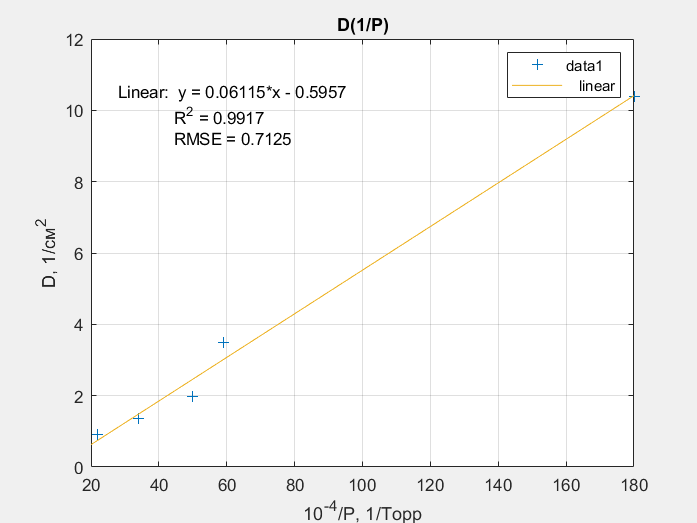
\includegraphics[width = 10.5 cm]{res}
    \label{fig:vac}
    
    \begin{center}
        \caption{$D(1/P)$}
    \end{center}
\end{figure} 

Из графика видно, что зависимость хороша аппроксимируется прямой ($R > 0,99$). 

Методом хи-квадрат найдём параметры графика:
\begin{equation}
    k = 611,1 \; \frac{\text{Торр} \cdot cm^2}{c}, \triangle k = 65,1 \; \frac{\text{Торр} \cdot cm^2}{c} 
\end{equation}

\begin{equation}
    b = 0,5957 \; \frac{cm^2}{c}, \triangle b = 0,0705 \; \frac{cm^2}{c} 
\end{equation}

Отсюда получим значение диффузии при атмосферном давлении: $D_P = 0.581 \; cm^2/c$, $\triangle D_P = 0.083 \; cm^2/c$

Сравним полученное значения с табличными. При температуре $273$ К значение коэффициента диффузии примеси гелия в воздухе составляет $0.66 \; cm^2/c$. То есть можно видеть, что в пределах погрешности полученное экспериментальное значение совпадает с теоретическим.

Оценим длину свободного пробега молекулы гелия по формуле 

\begin{equation}
    \lambda = \frac{3D}{\bar v}  = 3D \sqrt{\frac{\pi \mu }{8RT}} = 138 \text{ нм}
\end{equation}

При нормальных условиях табличное значение для длины свободного пробега молекулы гелия равно $180$ нм. Экспериментальное и теоретическое значения совпали по порядку величины.

Наконец, оценим эффективное сечение столконевний атомов гелия с частицами воздуха при температуре $300$ К и давлении $10^5$ Па:

\begin{equation}
    \lambda = \frac{\Delta V}{\sigma} = \frac{1}{n \sigma} = \frac{kT}{P \sigma} \Rightarrow \sigma = \frac{kT}{P \lambda} = 3,00 \cdot 10^{-19} \; \text{м}^2
\end{equation}

На самом деле эти рассуждения применимы, когда одна из молекул неподвижна. В случае относительного движения имеем значение, в $\sqrt{2}$ раза ниже полученного: $\sigma = 2,12 \cdot 10^{-19} \; \text{м}^2$

\newpage


\section{Заключение}

В ходе работы было экспериментально определено значение коэффициента диффузии для примеси гелия в воздухе. Был проведён эксперимент, при котором измерялась зависимость показаний вольтметра, соединённого с датчиком, определяющим разность концентраций примеси и основного газа. Полученные значения зависимости коэффициента диффузии от давления были экстраполированы к прямой и экспериментаьно было получено значение коэффициента диффузии при атмосферном давлении. Все значения были близки с теоретическим значениям.

Причины расхождения теории и эксперимента следующие: температура, при которой проводился эксперимент, была равна $300$ К, табличные значения определены для температуры $273$ К, то есть полученное значение получилось ниже, как и предсказывает закон Аррениуса (зависимость $D(T)$ в простом случае). Также следует учитывать, что при малейшем касании стола сбиваются настройки моста, из-за чего разность потенциалов почти постоянно была не точной (это можно видеть на построенных графиках).


\section{Список используемой литературы}

$\bullet$ Гладун А. Д. Лабораторный практикум по общей физике. Термодинамика и молекулярная физика\\

$\bullet$ \href{https://mipt.ru/education/chair/physics/S_II/lab/}{Описание лабораторных работ на кафедре общей физики МФТИ}

\newpage
\begin{figure}[h]
    \centering
    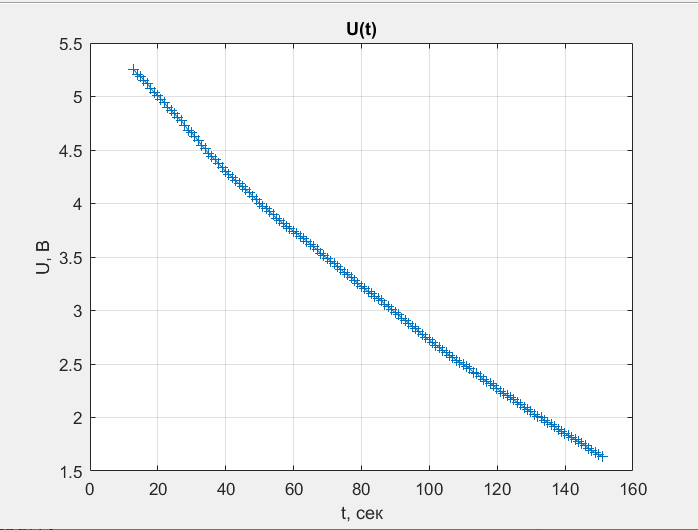
\includegraphics[width = 12 cm]{1gr55}
    \label{fig:vac}
    
    \begin{center}
        \caption{$P = 55$ Торр}
    \end{center}
\end{figure} 

\begin{figure}[h]
    \centering
    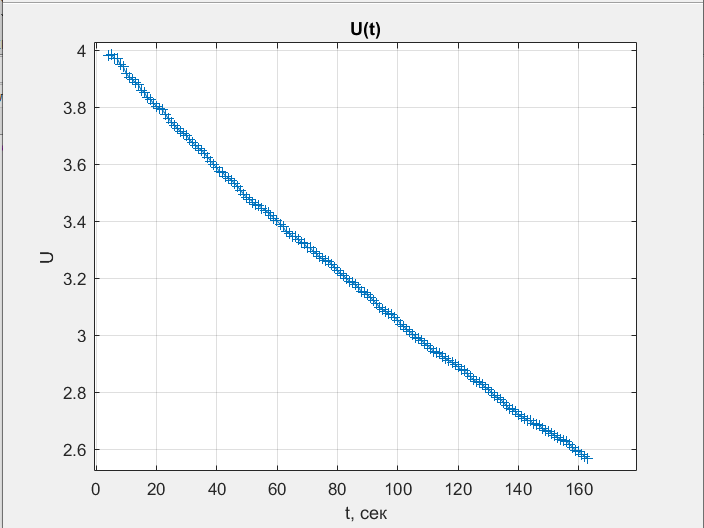
\includegraphics[width = 10.5 cm]{1gr169}
    \label{fig:vac}
    
    \begin{center}
        \caption{$P = 169$ Торр}
    \end{center}
\end{figure} 

\begin{figure}[h]
    \centering
    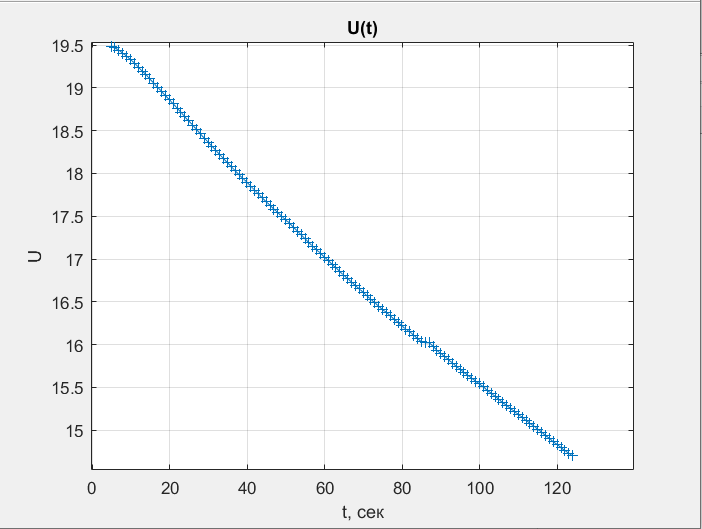
\includegraphics[width = 10.5 cm]{1gr200}
    \label{fig:vac}
    
    \begin{center}
        \caption{$P = 200$ Торр}
    \end{center}
\end{figure} 

\begin{figure}[h]
    \centering
    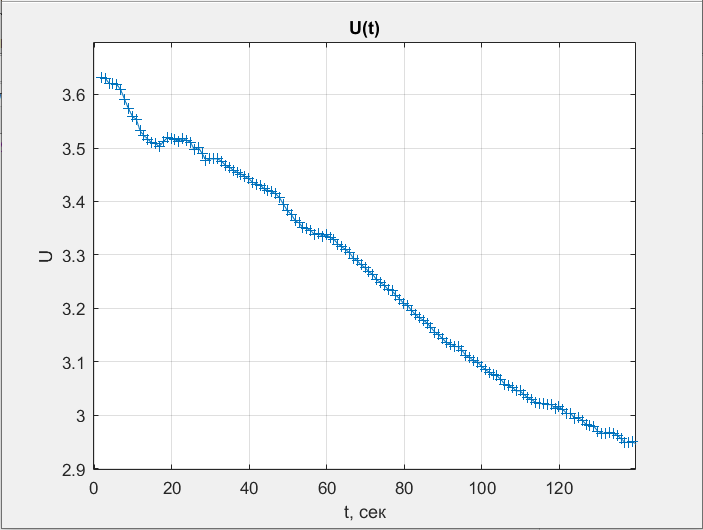
\includegraphics[width = 10.5 cm]{1gr293}
    \label{fig:vac}
    
    \begin{center}
        \caption{$P = 293$ Торр}
    \end{center}
\end{figure} 

\begin{figure}[h]
    \centering
    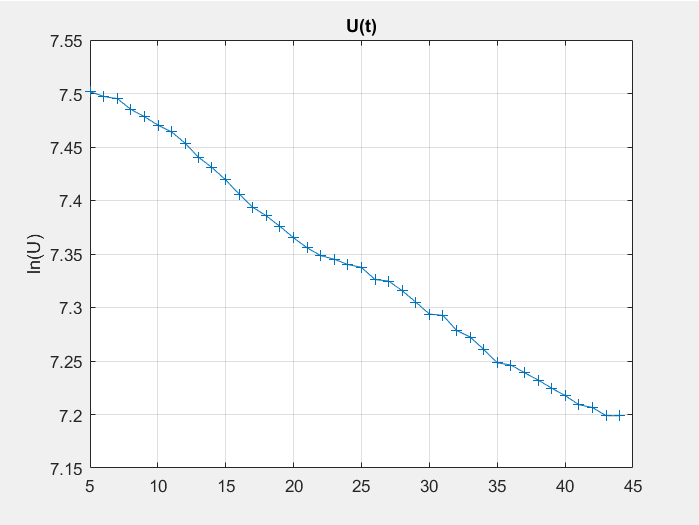
\includegraphics[width = 10.5 cm]{1gr447}
    \label{fig:vac}
    
    \begin{center}
        \caption{$P = 447$ Торр}
    \end{center}
\end{figure} 

\begin{figure}[h]
    \centering
    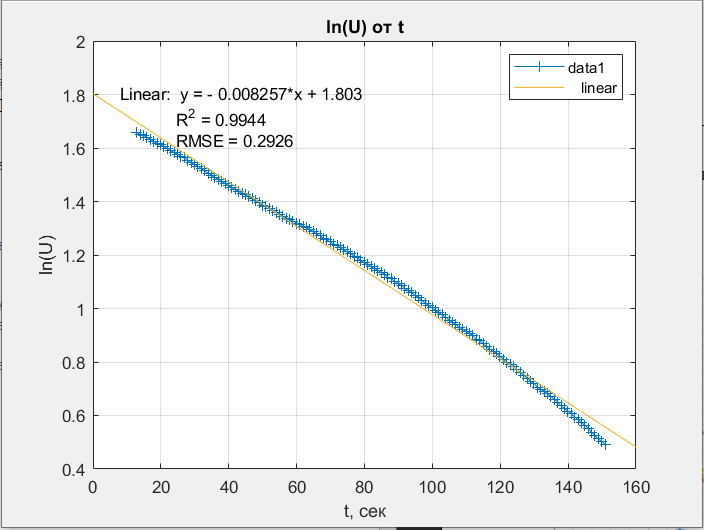
\includegraphics[width = 10.5 cm]{2gr55}
    \label{fig:vac}
    
    \begin{center}
        \caption{$P = 55$ Торр}
    \end{center}
\end{figure} 

\begin{figure}[h]
    \centering
    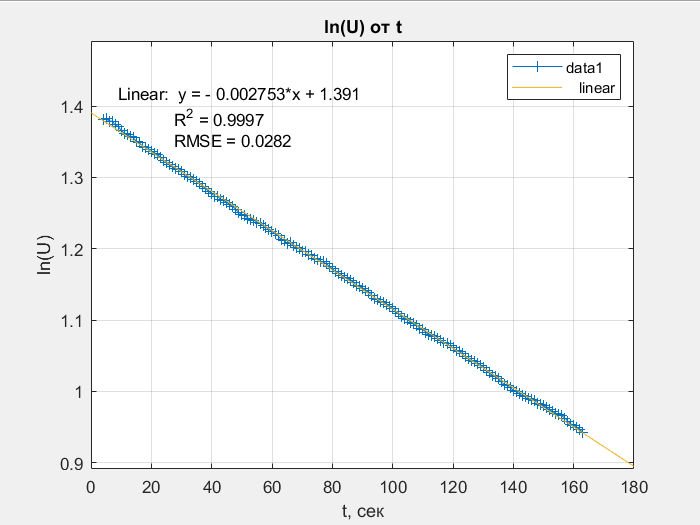
\includegraphics[width = 10.5 cm]{2gr169}
    \label{fig:vac}
    
    \begin{center}
        \caption{$P = 169$ Торр}
    \end{center}
\end{figure} 

\begin{figure}[h]
    \centering
    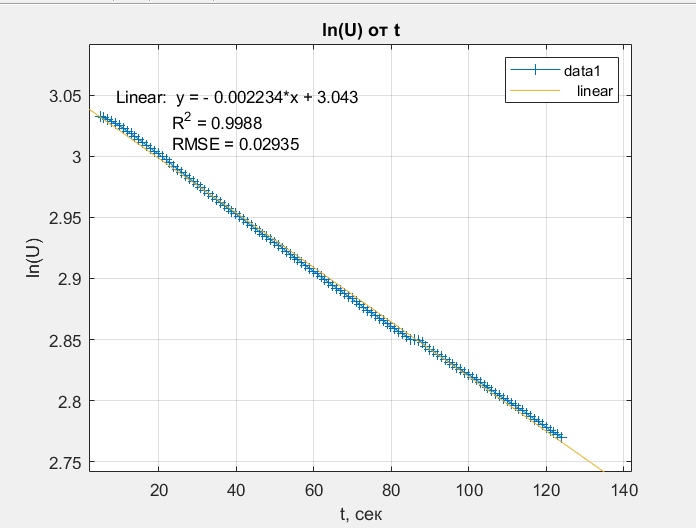
\includegraphics[width = 10.5 cm]{2gr200}
    \label{fig:vac}
    
    \begin{center}
        \caption{$P = 200$ Торр}
    \end{center}
\end{figure} 

\begin{figure}[h]
    \centering
    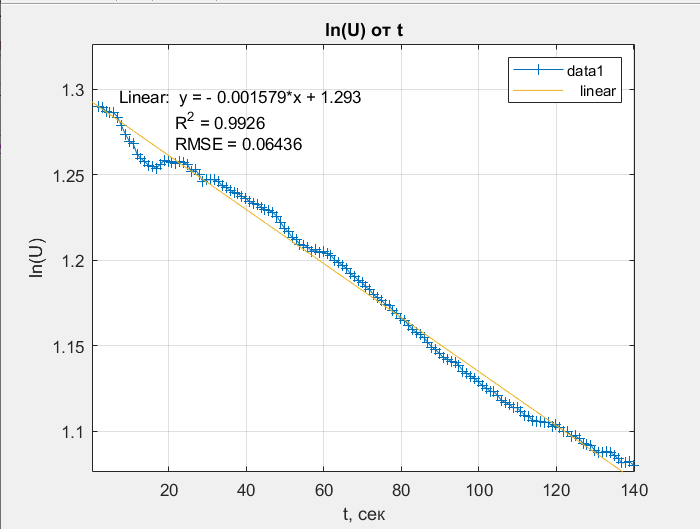
\includegraphics[width = 10.5 cm]{2gr293}
    \label{fig:vac}
    
    \begin{center}
        \caption{$P = 293$ Торр}
    \end{center}
\end{figure} 

\begin{figure}[h]
    \centering
    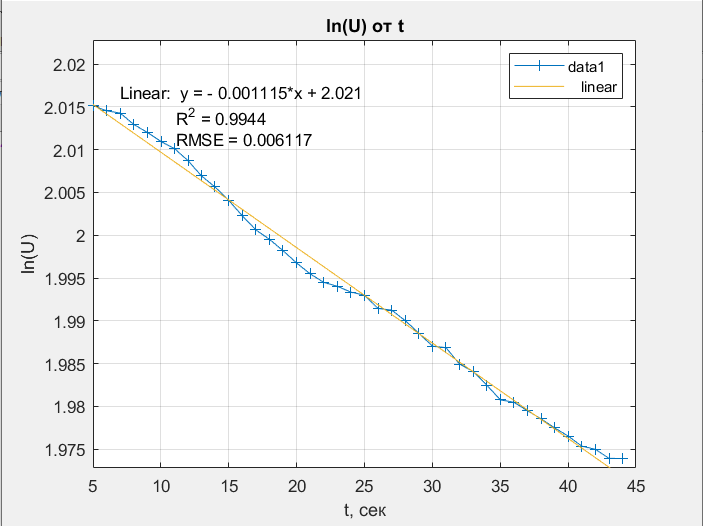
\includegraphics[width = 10.5 cm]{2gr447}
    \label{fig:vac}
    
    \begin{center}
        \caption{$P = 447$ Торр}
    \end{center}
\end{figure} 

\end{document}